%%%%%%%% ICML 2025 EXAMPLE LATEX SUBMISSION FILE %%%%%%%%%%%%%%%%%

\documentclass{article}

% Recommended, but optional, packages for figures and better typesetting:
\usepackage{microtype}
\usepackage{graphicx}
\usepackage{subfigure}
\usepackage{booktabs} % for professional tables

% hyperref makes hyperlinks in the resulting PDF.
% If your build breaks (sometimes temporarily if a hyperlink spans a page)
% please comment out the following usepackage line and replace
% \usepackage{icml2025} with \usepackage[nohyperref]{icml2025} above.
\usepackage{hyperref}


% Attempt to make hyperref and algorithmic work together better:
\newcommand{\theHalgorithm}{\arabic{algorithm}}
\newcommand{\algorithmautorefname}{Algorithm}

% Use the following line for the initial blind version submitted for review:
% \usepackage{icml2025}

% If accepted, instead use the following line for the camera-ready submission:
\usepackage[accepted]{icml2025}

% For theorems and such
\usepackage{amsmath}
\usepackage{amssymb}
\usepackage{mathtools}
\usepackage{amsthm}

% if you use cleveref..
\usepackage[capitalize,noabbrev]{cleveref}

%%%%%%%%%%%%%%%%%%%%%%%%%%%%%%%%
% THEOREMS
%%%%%%%%%%%%%%%%%%%%%%%%%%%%%%%%
\theoremstyle{plain}
\newtheorem{theorem}{Theorem}[section]
\newtheorem{proposition}[theorem]{Proposition}
\newtheorem{lemma}[theorem]{Lemma}
\newtheorem{corollary}[theorem]{Corollary}
\theoremstyle{definition}
\newtheorem{definition}[theorem]{Definition}
\newtheorem{assumption}[theorem]{Assumption}
\theoremstyle{remark}
\newtheorem{remark}[theorem]{Remark}

% Todonotes is useful during development; simply uncomment the next line
%    and comment out the line below the next line to turn off comments
% \usepackage[disable,textsize=tiny]{todonotes}
\usepackage[textsize=tiny]{todonotes}

% Package for fancy math letters
\usepackage{dsfont}

% The \icmltitle you define below is probably too long as a header.
% Therefore, a short form for the running title is supplied here:
\icmltitlerunning{Another fun title to think of...}

\begin{document}

\twocolumn[
\icmltitle{Tabular Reinforcement Learning : Catchy title pending}

% It is OKAY to include author information, even for blind
% submissions: the style file will automatically remove it for you
% unless you've provided the [accepted] option to the icml2025
% package.

% List of affiliations: The first argument should be a (short)
% identifier you will use later to specify author affiliations
% Academic affiliations should list Department, University, City, Region, Country
% Industry affiliations should list Company, City, Region, Country

% You can specify symbols, otherwise they are numbered in order.
% Ideally, you should not use this facility. Affiliations will be numbered
% in order of appearance and this is the preferred way.
\icmlsetsymbol{equal}{*}

\begin{icmlauthorlist}
\icmlauthor{Ali Momen (s4993128)}{LU}
\icmlauthor{Bram Bouma (s2646072)}{LU}
\icmlauthor{Judith Moulijn (s3206025)}{LU}
\end{icmlauthorlist}

\icmlaffiliation{LU}{Universiteit Leiden, The Netherlands}
%\icmlaffiliation{comp}{Company Name, Location, Country}
%\icmlaffiliation{sch}{School of ZZZ, Institute of WWW, Location, Country}

\icmlcorrespondingauthor{Ali Momen}{amomen@gmail.com}
\icmlcorrespondingauthor{Bram Bouma}{bram.f.bouma@gmail.com}
\icmlcorrespondingauthor{Judith Moulijn}{j.moulijn@umail.leidenuniv.nl}

% You may provide any keywords that you
% find helpful for describing your paper; these are used to populate
% the "keywords" metadata in the PDF but will not be shown in the document
\icmlkeywords{Tabular Reinforcement Learning}

\vskip 0.3in
]

% this must go after the closing bracket ] following \twocolumn[ ...

% This command actually creates the footnote in the first column
% listing the affiliations and the copyright notice.
% The command takes one argument, which is text to display at the start of the footnote.
% The \icmlEqualContribution command is standard text for equal contribution.
% Remove it (just {}) if you do not need this facility.

%\printAffiliationsAndNotice{}  % leave blank if no need to mention equal contribution
\printAffiliationsAndNotice{\icmlEqualContribution} % otherwise use the standard text.


\newpage
\begin{abstract}

This article is about implementing Reinforcement Learning various algorithms on a grid world problem with stochastic factors. The algorithms are run in enough explained iterations to use the previous learnings, to be able to converge to the terminal state in less steps. Every algorithm is also run multiple times to generate more results so as to be more reliably comparable with the other algorithms. The approaches and algorithms included are "\textbf{Dynamic Programming}", "\textbf{Exploration Techniques}", "\textbf{On-policy versus Off-policy}", "\textbf{Depth of Target}".
\end{abstract}

\section{Introduction} \label{sec:introduction}
Finding an optimal path in a given situation can be modeled using tabular reinforcement learning (RL). In this regime of RL the state and actions spaces are discrete. Relatively low-dimensional "grid worlds" in this regime allow for both state and action spaces to be stored in their entirety. Here we will cover several methods for finding the optimal path through a certain environment.  

In \autoref{sec:theory} the theory relevant for the methods used is covered. This will be based on the work in \cite{RL_book}.
In \autoref{sec:experiments} the different experiments applied to find the optimal path through this environment are covered and their results are presented. In \autoref{sec:discussion} these results are discussed. We end with a reflection in \autoref{sec:conclusion}

\section{Theory}\label{sec:theory}
Let's cover some terms that will be used throughout this work. An agent will make a sequence of actions to traverse an environment and reach a goal. Such a problem is therefore also called a Sequential Decision Problem (SDP). Though in real life, humans often let their experience of previous decisions lead their following decisions this is not the case in Markov Decisions Processes (MDPs). In MDPs the next action taken is solely based on the information available at a given state. By tackling an SDP using an MDP allows us to straightforwardly model an agent's behaviour. Taking all past experiences into account, becomes complicated. To model an SDP as an MDP the following things are needed: the actions the agent can take (the action space $A$), the states the environment can be in (the state space $S$), the rewards associated with each state $r_s$, the probability to transition from one state ($s$) to another ($s'$), given an action ($a$) denoted by $T(s'|a,s)$ and a discount factor $\gamma$ which decides how much future possible rewards are weighted into the decision making process. So how do we use this information to decide what are good actions to take? First we need to know what the return $R$ means. It is given by the following equation:
\begin{equation}
    R = \sum_{i=0}^N r_i \gamma^i
    \label{eq:return}
\end{equation}
With $N$ the number of steps taken by the agent and $r_i$ the reward received at time step $i$. This leads us to the state-action value function $Q(s,a)$. This is the expected return $R$ if a given policy $\pi(a|s)$ is used to decide what action to take after being in state $s$ and taking action $a$. Or, in equation form
\begin{equation}
    Q^\pi(s,a) = \mathds{E}\left[\sum_{i=0}^N\gamma^i \cdot r_{t+i}|s_t=s,a_t=a\right]
    \label{eq:state_action_value}
\end{equation}
With $r_t$ the reward received, $s_t$ the environment state and $a_t$ the action taken at timestep $t$. The goal is to find the optimal policy which maximises this expected return, or
\begin{equation}
    \pi^\star = \arg\max_{a\in A} Q^\star(s,a)
    \label{eq:RL_goal}
\end{equation}

\section{Experiments}\label{sec:experiments} %(setup and results)
Let's now go over the environment that will be used throughout this report. The environment in which the agent is moving around is a 7x10 grid world. The agent starts at a starting position (0,3). A goal location is set at (7,3) and can be moved around. Reaching the goal state yields a reward of $100$. Reaching any other state yields a reward of $-1$. In columns 3, 4, 5 and 8 there's a 90\% change that the agent will be moved upwards one tile, due to a stochastically present wind. In columns 6 and 7 this results in an upwards movement of two tiles with the same probability.

\subsection{Dynamic programming}\label{subsec:dynamic_programming}
A method of constructing the state-action value function $Q(s,a)$ is by using the Value Iteration algorithm (see \autoref{alg:Q_value_iteration}). This algorithm loops over both state and action spaces to iteratively improve the $Q$ table using \autoref{eq:dynamic_programming_Q_table} until the state-actions values don't change much anymore (convergence is reached). 

\begin{equation}
    Q(s,a) \leftarrow \sum_{s'}\left[p(s'|s,a) \cdot \left(r(s,a,s') + \\ \gamma \max_{a'}Q(s',a')\right)\right]
    \label{eq:dynamic_programming_Q_table}
\end{equation}
Where $p(s'|s,a)$ is the transition probability mentioned in \autoref{sec:theory}.

The output of \autoref{alg:Q_value_iteration} is an optimal (within the constraints of the parameters used) $Q$ table which can be used to help the agent reach the goal. In a given state $s$, the next action $a'$ is chosen based on the action that maximises the $Q(s,a')$ value. This is called a \textit{greedy} policy. This algorithm requires the transition probability to be known from the environment and is therefore a model-based solution method for the MDP. 


The converged optimal value at the start state can be found using the value function \cite{RL_book}:
\begin{equation}
    V^\pi(s) = \mathds{E}\left[\sum_{i=0}^N \gamma^i \cdot r_{t+i}|s_t = s \right]
    \label{eq:value_function}
\end{equation}
With $\gamma$ the discount factor and $N$ the number of steps taken until the goal is reached. This can be used in $V(s_\text{initial})$ to get an expected return for the entire episode (from the initial state up to when the goal is reached).

\subsubsection{Hyperparameters}
The main hyperparameters used in this experiment are the discount factor $\gamma$ and the threshold $\eta$. Setting $\gamma$ lower will mean that the $Q$ table is built up by taking only the closest rewards into account (see also \autoref{fig:DP_low_gamma}). Setting $\gamma$ equal to one, means all future rewards are taken into account equally. Setting $\eta$ higher means that convergence is reached earlier. If the steps to states other than the terminal state awarded $0$ instead of $-1$, the shorted path could still be found using $\gamma<1$. By only considering a few states ahead too much exploring is discouraged: this will yield no reward.

\subsubsection{Results}
Using $\gamma=0.99$ and $\eta=70.$ \autoref{alg:Q_value_iteration} converges in 12 iterations. Then applying \autoref{eq:value_function} on the initial state yields $V(s_\text{initial})\approx 70$. We can also calculate the average reward per timestep using the reward in the terminal state ($R_\text{terminal}$), the fact that each step to a different state yields a reward of $-1$ and the number of steps taken ($N_\text{steps}$). The average reward per timestep is then
\begin{equation}
    \bar{r_t} = \left(100 + (n_\text{steps}-1)\cdot -1\right)/n_\text{steps}
    \label{eq:average_reward_per_timestep}
\end{equation}
A single step is subtracted from $n_\text{steps}$ inside the equation because the final step into the terminal state doesn't yield a reward of $-1$ but one of $100$ as previously stated.
On average, using the same values for the hyperparameters $\gamma$ and $\eta$, it takes about 17 steps to reach the terminal state. This means that $\bar{r_t}\approx 4.9$.

\begin{figure}[H]
     \centering
     
\includegraphics[width=\linewidth]{Figures/step1_VI_at_end.pdf}
     \caption{After 12 iterations of value iteration, convergence is reached (when using $\gamma=0.99$ and $\eta=70.$). For ealier stages of the algorithm see \autoref{fig:value_iteration_beginning} and \autoref{fig:value_iteration_halfway}. The agent will move to the right, end up in the top-right corner due to the stochastic wind, then work its way to the bottom-right and then to the left and up towards the goal.} 
     \label{fig:value_iteration_end}
 \end{figure}

\subsection{Exploration}\label{subsec:exploration}
The exploration experiment is all about choosing the action (select\_action) in the current state, either the same as the previous trials (greedy) or choosing a new action with a risk factor. The selection between these two is performed in 2 "\textbf{e-greedy}" and "\textbf{Boltzman (softmax)}" methods. The stochasticity is applied through one of these methods. Then we compare how these two methods relatively perform by drawing a plot. 


Here is the action selection policy formula for the \textbf{e-greedy} method:
\[
\pi(a \mid s)=
\begin{cases}
1.0 - \epsilon \cdot \dfrac{|A|-1}{|A|}, 
& \text{if } a=\arg\max_{b\in A}\hat{Q}(s,b):\space\ Exploitation \\[6pt]
\dfrac{\epsilon}{|A|}, 
& \text{otherwise}:\space\space\space Exploration
\end{cases}
\]
The upper case covers exploitation and the lower case covers exploration which chooses 1 from the rest of non-greedy actions. And the action selection policy formula for the \textbf{Boltzman} method:
\[
\pi(a \mid s)=
\frac{e^{\hat{Q}(s,a)/\tau}}
{\sum_{b\in A} e^{\hat{Q}(s,b)/\tau}}
\]
 It also gives a probability to every possible action.
 

\subsubsection{Hyperparameters}
The hyperparameters in experiments generally include \textbf{learning rate $\alpha$}, \textbf{exploration rates} $\epsilon$ and $\tau$ for e-greedy and softmax methods respectively, \textbf{number of timesteps} (budget), $\gamma$ (\textbf{discount factor}), and \textbf{evaluation interval}. We try to tune them as far as we can. The hyperparameters and figures for the first and last trials are in the appendix section, and I only do the final interpretation here.
\paragraph{Hyperparameters Optimization} (Numerical discussion in the Appendix section)
The initial number of timesteps (50001) was too large for the need (tangible convergence), and it could be reasonable to start with a bigger value, and then decrease it after observing the results, but subsequently we decreased it. Also, a faster convergence was obviously more desirable so we tried to increase learning rate and adjust the exploration rates accordingly. Increasing the learning rate and keeping other parameters static, as expected lead to two results:
1. Faster convergence
2. Volatile behavior of some curves, slow convergence (less curve slope), oscillation, and less satisfactory \textbf{Returns}
We reacted to this by decreasing the exploration rates. This fixed the  problem. Meaning the curves not only converged faster (less timesteps), but also had steady and smooth behavior. The evaluation interval was not changed to keep the plots smoother (Numerical discussion in the Appendix section).

\begin{itemize}
    \item We also added another goal to the environment with a different reward value. It is also a terminal state, so when the \textbf{Agent} reaches it, the movement stops. This obviously changes the curve. We took the positions [3,2], [7,4], and [8,4] one at a time (3 experiments) for the second goal and a reward value of 5. The change is that the mean of returns, convergence speed, and hyperparameter effects change. But everything depends so much on where the second goal, and what its reward value are. If it is generally much more likely to be visited, then the Returns will orient so much to it reward value. Further discussion in the Appendix due to the space limitation. 
\end{itemize}


\subsection{Back-up: On-policy versus off-policy target}\label{subsec:backup_on_off}

An important aspect that influences the process of tabular reinforcement learning is the way that the state-action value function is updated. There are two ways to execute this back-up. The first is off-policy, where a bootstrapped value is given by the best possible next action, according to the Q-table. This is how the Q-learning algorithm works (see \autoref{alg:tabular_q_learning}). The other way is on-policy, where the value is not determined by the best possible action, but by the action actually taken by the agent. This approach is used by the RL algorithm SARSA (see \autoref{alg:SARSA}). After initializing, SARSA takes actions based on the current policy and observes the resulting next state and reward. Then, the Q-value of the current state-action pair is updated, using the action taken by the agent.

 \begin{figure}[H]
     \centering
     
\includegraphics[width=\linewidth]{Figures/on_off_policy.pdf}
     \caption{Comparing different approaches of target back-up. Q-learning uses an off-policy back-up with and SARSA uses an on-policy back-up. Both algorithms are tested with learning rates 0.03, 0.1 and 0.3.} 
     \label{fig:off_on_policy}
 \end{figure}

\subsection{Back-up: Depth of target}\label{subsec:backup_depth}

When considering back-up, deciding on off-policy versus on-policy is not the only choice that impacts the performance of the agent. So far, when computing the target value, only the next action was taken into consideration. The agent was only looking one step forward, so to speak. But, it is also possible to look further ahead before bootstrapping, summing rewards into a trace with a discount for rewards that lie further in the future. These methods are known as N-step methods, with depth n denoting how many step the agent looks into the future. One of these is N-step Q-learning (see \autoref{alg:N_step_q_learning}). It collects a full episode before updating the Q-value of each encountered state-action pair, summing over the discounted rewards.

An extreme case of N-step Q-learning is the Monte Carlo update, where the update uses the sum of all discounted rewards until the end of the episode, without any bootstrapping. The algorithm for this approach is shown in \autoref{alg:Monte_Carlo}. Just like the N-step Q-learning algorithm, this algorithm first collects a full episode and then loops backwards through the encountered state-action pairs, accumulating the sum of discounted rewards in reverse and updating the Q-table accordingly.



 \begin{figure}[H]
     \centering
     
\includegraphics[width=\linewidth]{Figures/depth.pdf}
     \caption{Comparing different back-up depths using depths of 1, 3, 10 steps and a Monte Carlo update, which considers all steps up to the end of the episode.} 
     \label{fig:back_up_depth}
 \end{figure}

\section{Discussion}\label{sec:discussion}
\todo{Curse of dimensionality}
\subsection{Dynamic programming}\label{subsec:discussion_dynamic_programming}
The optimal $Q$ table found using $\gamma=0.99$ and $\eta=70.$ is visualised in \autoref{fig:value_iteration_end}. The blue square indicates the initial state and the green square indicates the terminal state. The arrows indicate the greedy action to take in each state. No reward can be received after the agent reaches the goal state: no action is preferred so each action is indicated with an arrow. To ensure that the agent doesn't move away from the goal state, the transition probability is defined such that each action from the goal state will return the goal state: no movement away from the goal state is permitted. Changing the goal state will yield a different $Q$ table, because different actions will be required to reach this changed goal state (see for example \autoref{fig:DP_other_goal}). 

Using \autoref{alg:Q_value_iteration} to find the optimal policy $\pi^\star$ works well \textbf{if} we can afford its high computational cost and we have access to $T(s'|a,s)$.


\subsection{Exploration}\label{subsec:discussion_exploration}
 For choosing the exploration method, it boils down to what values we choose for $\epsilon$ and $\tau$. If they are chosen well enough, there is not much performance difference between these two methods. Since I changed both to get a relatively optimal result, I will note my selected values in the Appendix section.
When we turn the reward value for the goal to 0, I believe the convergence will occur with the same speed, though the mean of returns will be different and for high values like 100, the curve goes upwards with a large slope and at some point it becomes descending, and in conclusion, I do not believe changing the rewards would have so much effect on the convergence, so long as the goal reward value is bigger than the other steps 
Questions from assignment: \\

\subsection{ Back-up: On-policy versus off-policy target}\label{subsec:discussion_backup_on_off}

Considering the comparison of Q-learning and SARSA for different learning rates in \autoref{fig:off_on_policy}, the off-policy Q-learning approach with a learning rate of 0.1 seems to yield the highest return with the most consistency, implying that the off-policy approach of updating with the best action results in better training of the agent due to the direct learning of the optimal policy, whereas SARSA accounts for more exploration, learning a suboptimal but more realistic policy.
The on-policy (SARSA) approach would be more useful in the case that exploration is dangerous, and the safest path to the reward is the way to go.

A learning rate of 0.1 seems to balance stability and learning speed, as a lower $\alpha$ would converge to slow and a higher $\alpha$ would overshoot the values in the Q-table. Note that for the same learning rates the learning curves of Q-learning and SARSA look similar, indicating that the learning rate dominated the learning process compared to the approach used to update the Q-table.

\subsection{Back-up: Depth of target}\label{subsec:discussion_backup_depth

\autoref{fig:back_up_depth} shows the comparison between different back-up depths for N-step Q-learning, compared to the Monte Carlo approach. The figure shows the highest return for the depths of $n=1$ and $n=3$, with the 1-step approach learning the fastest initially, propagating information at every timestep, but the 3-step approach catching up quickly for more timesteps. For $n=3$, the target value includes more information about future rewards, so it has less bias than for $n=1$ (which only uses 1 real reward) but it takes longer to see improvements because fewer updates are happening per timestep, leading to the fast increase later. For $n=10$ or larger, the target update becomes to noisy, with a high variance, considering that the environment is stochastic, leading to a worse performance. But , when given enough time to converge, 10-step Q-learning has the potential to reach the optimal policy, since it uses 10 actual rewards before bootstrapping, resulting in a low bias and the most consistent rising learning curve, in contrast to the learning curves for $n=1$ and $n=3$, for which the return decreases again at about 30000 timesteps.

When compared to \autoref{fig:off_on_policy}, the 1-step Q-learning seems to learn slower then when executing \autoref{alg:tabular_q_learning}. This could be because regular Q-learning updates every single timestep, while 1-step Q-learning collects a full episode first and only then updates.

Coming back to on-policy versus off-policy, the N-step approach lies somewhere in between. The first n rewards are collected using the on-policy approach, resulting in a trace of rewards that reflect the current policy. But, when bootstrapping, the update uses $\text{max}_a \hat{Q}(s_{t+m}, a)$, just like in regular Q-learning.

\section{Conclusion}\label{sec:conclusion}


%Include the bibliography
\bibliography{bibliography}
\bibliographystyle{icml2025}



%Include an appendix
\newpage
\appendix

\section{Algorithms}\label{app:algorithms}

\subsection{Dynamic programming}
Below is the pseudocode for the value iteration algorithm used to construct the $Q$-table in \autoref{subsec:dynamic_programming}.
\begin{algorithm}[H]
   \caption{Tabular Q-value iteration}
   \label{alg:Q_value_iteration}
\begin{algorithmic}
   \STATE {\bfseries Input:} $n_\text{states}$, $n_\text{actions}$, threshold $\eta \in\mathrm{R}_{>0}$
   \STATE \textbf{Initialise:} A state-action value table $Q$ with shape $(n_\text{states},n_\text{actions})$ and $Q(s,a)=0$ $\forall s\in S, a \in A$
   \STATE \textbf{Output:} Optimal state-action value table $Q^\star$
   \REPEAT
   \STATE $\Delta$ $\leftarrow$ 0
   \FOR{each $s \in S$}
   \FOR{each $a \in A$}
   \STATE $x \leftarrow Q(s,a)$ \\
   \STATE $\tilde{Q}(s,a) \leftarrow \sum_{s'}[p(s'|s,a) \cdot (r(s,a,s')+$
   \STATE $\gamma \cdot \max_{a'}Q(s',a'))]$ \\
   \STATE $\Delta \leftarrow \text{max}\left(\Delta,|x - \tilde{Q}(s,a)|\right)$
   \ENDFOR
   \ENDFOR
   \UNTIL{$\Delta < \eta$}
\end{algorithmic}
\end{algorithm}

\subsection{Exploration}
This is the general pesudo-code implemented for the Q-Learning method as mentioned in \autoref{subsec:exploration}:

\begin{algorithm}[H]
   \caption{Tabular Q-learning}
   \label{alg:tabular_q_learning}
\begin{algorithmic}
   \STATE \textbf{Input:} exploration parameter, learning rate $\alpha \in (0,1]$, discount factor $\gamma \in [0,1]$, total budget
   \STATE \textbf{Initialise:} $\hat{Q}(s,a)\leftarrow 0,\ \forall s\in S,\ a\in A$
   \STATE $s \sim p_0(s)$ \hfill /* sample initial state */
   \WHILE{budget not exhausted}
      \STATE $a \sim \pi(a\mid s)$ \hfill /* e.g., $\epsilon$-greedy, softmax */
      \STATE $r,s' \sim p(r,s' \mid s,a)$ \hfill /* simulate environment */
      \STATE $\hat{Q}(s,a)\leftarrow \hat{Q}(s,a)+\alpha\left[r+\gamma\max_{a'}\hat{Q}(s',a')-\hat{Q}(s,a)\right]$
      \IF{$s'$ is terminal}
         \STATE $s \sim p_0(s)$ \hfill /* reset environment */
      \ELSE
         \STATE $s \leftarrow s'$
      \ENDIF
   \ENDWHILE
   \STATE \textbf{Return:} $\hat{Q}(s,a)$
\end{algorithmic}
\end{algorithm}

As mentioned in the body of the report, the \textbf{Experimentation} part, here comes some plots and debates.
These are sample snapshots of the running environments:
With one goal:
\begin{figure}
    \centering
    
\includegraphics[width=0.5\linewidth]{Screenshot_99.png}
    \caption{Agent moving with the environment in the 1 goal scenario. Preferable actions are show after every step-out}
    \label{fig:placeholder}
\end{figure}
\begin{figure}
    \centering
    
\includegraphics[width=0.5\linewidth]{Screenshot_98.png}
    \caption{Agent moving with the environment in one of 2 goals scenarios. Preferable actions are show after every step-out}
    \label{fig:placeholder}
\end{figure}
\paragraph{Hyperparameters}

These are the original values for the following hyperparameters:
    n_timesteps = 50001
    eval_interval = 1000
    max_episode_length = 100
    gamma = 1.0
    epsilons = [0.03,0.1,0.3]
    learning_rate = 0.1
    temps = [0.01,0.1,1.0]
Resulting Graph:
\begin{figure}
    \centering
    
\includegraphics[width=0.5\linewidth]{exploration_lr0p1_eps0p03-0p1-0p3_temp0p01-0p1-1_rep20_ts50001_eval1000_1.png}
    \caption{Original hyperparameters graph}
    \label{fig:placeholder}
\end{figure}
The values gradually changed for all learning rate, temperatures, and epsilon values to:
    n_timesteps = 15001
    eval_interval = 1000
    max_episode_length = 100
    gamma = 1.0
    epsilons = [0.00001,0.0001,0.001] 
    learning_rate = 0.7
    temps = [0.0001,0.001,0.01] 
Result:
\begin{figure}
    \centering
    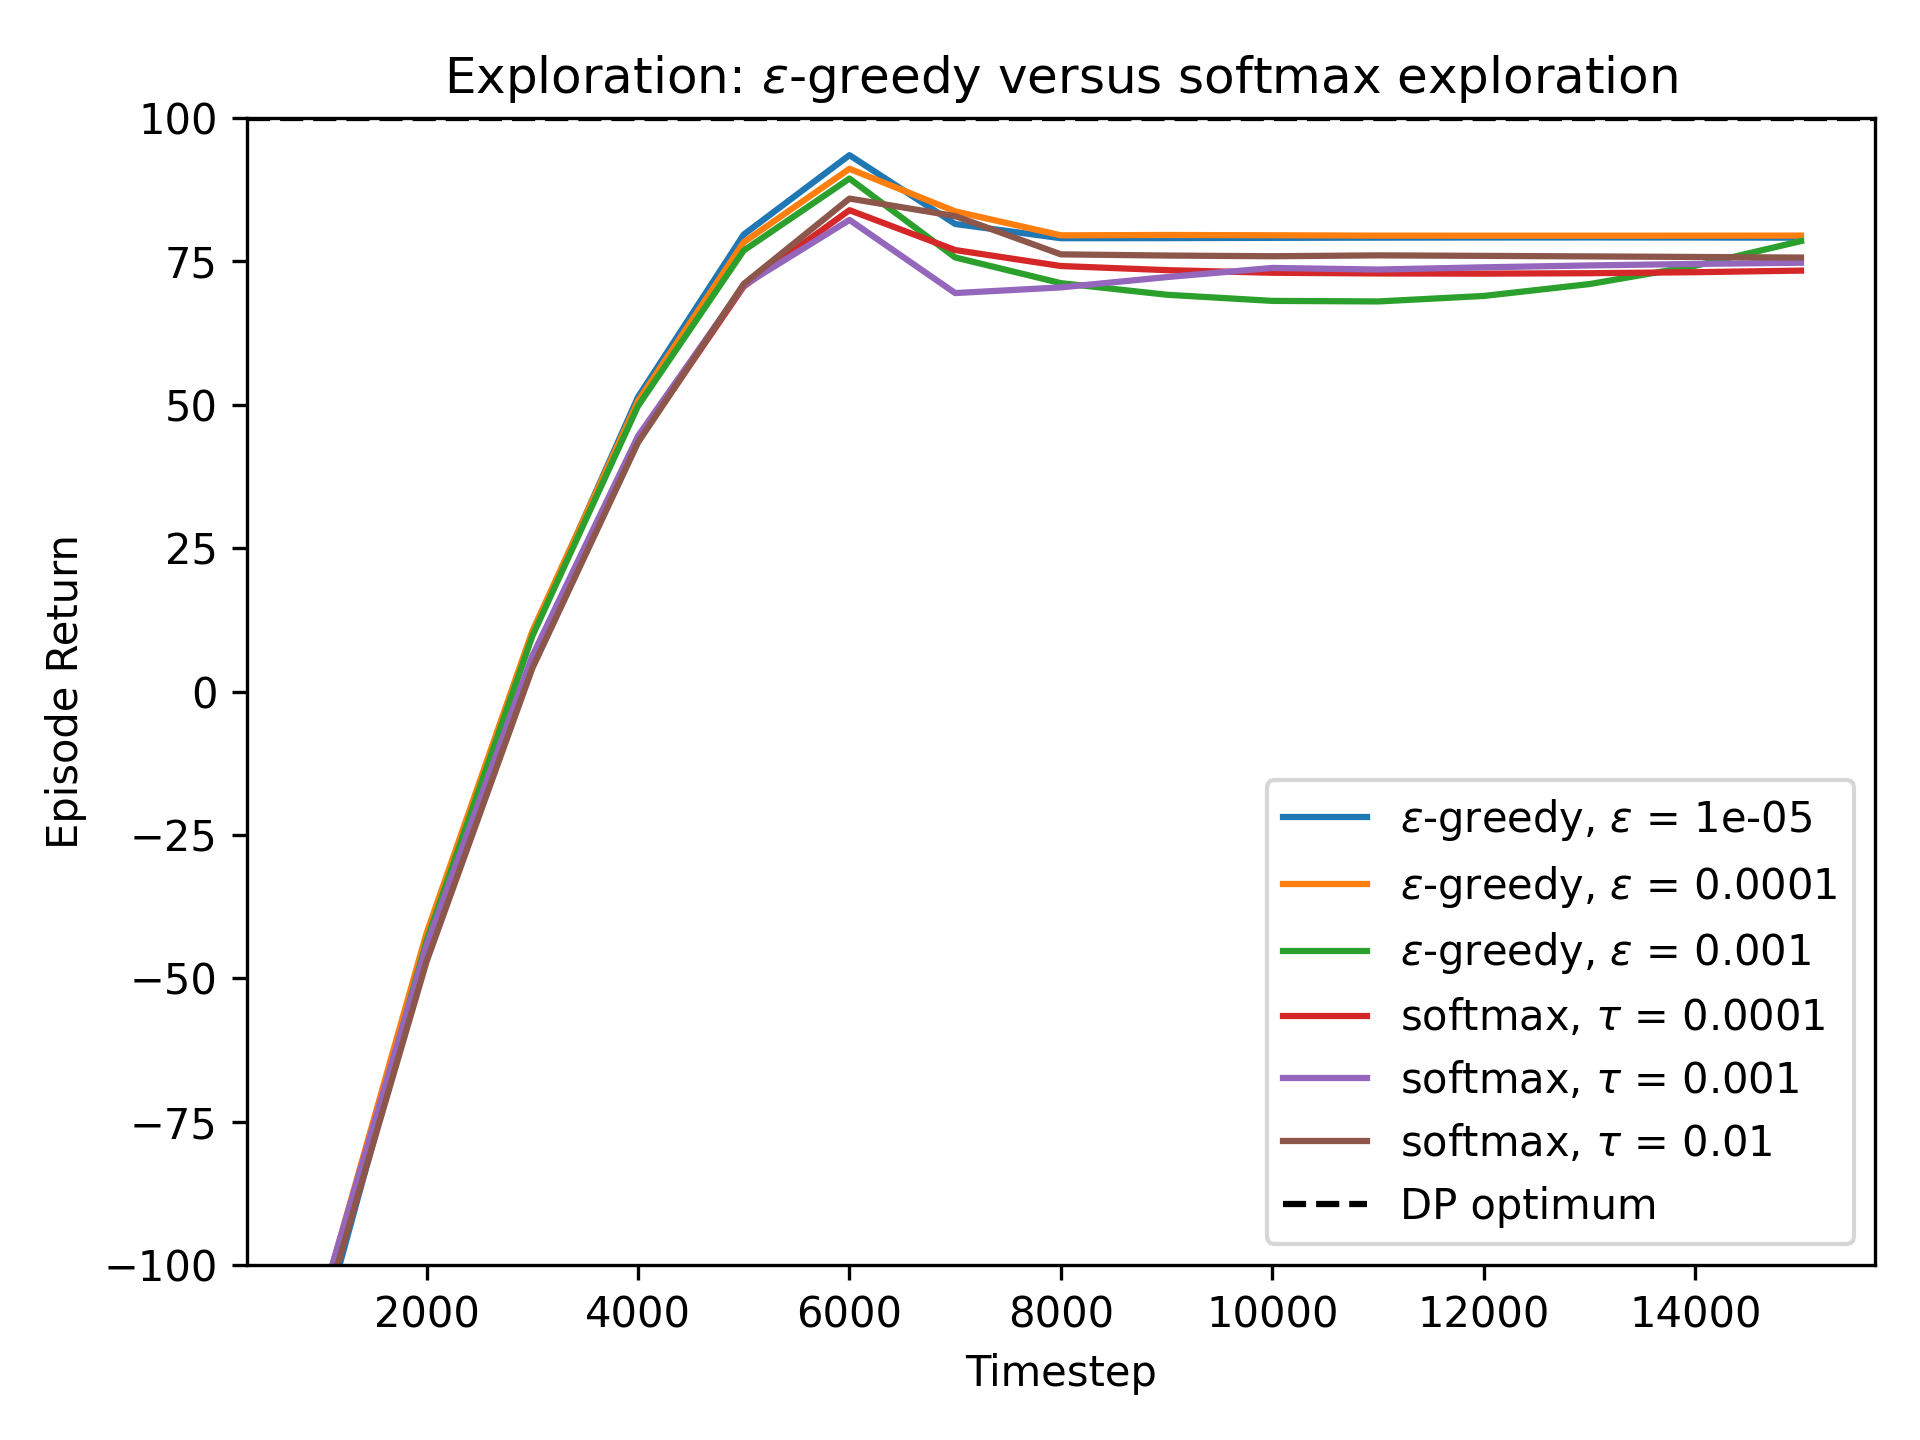
\includegraphics[width=0.5\linewidth]{exploration_lr0p7_eps1e-05-0p0001-0p001_temp0p0001-0p001-0p01_rep20_ts15001_eval1000.png}
    \caption{Graph with the new assigned hyperparameters}
    \label{fig:placeholder}
\end{figure}
The number of n_timestamps has decreased from 50001 to 15001, because the graph converged much faster. The oscillations and volatile behaviors have also significantly decreased. This also demonstrates that the performance of the two $\epsilon$ greedy and softmax boils down to proper choice of the $\epsilon$ and $\tau$ values. More graphs exist in the Exploration_plots of the assignment repository.
\textbf{Two Goals:}
As for the two goals, I tried the following locations for the second goal: 
[3,2], [7,4], and [8,4]
They are also terminal states, so
when the Agent reaches it, the movement stops. This
obviously changes the curve so much. We took the positions
 one at a time (3 experiments)
for the second goal and a reward value of 5. The
change is that the mean of returns, convergence speed,
and hyperparameter effects change. But everything
depends so much on where the second goal, and what
its reward value are. If it is generally much more likely
to be visited, then the Returns will orient so much to its
reward value. Here are the three respective Graphs with their respective tuned hyperparameters.
\begin{figure}
    \centering
    
\includegraphics[width=0.5\linewidth]{exploration_2Goals(7332)_lr0p1_eps0p03-0p1-0p3_temp0p01-0p1-1_rep20_ts15001_eval1000.png}
    \caption{Goal1: [7,3]
    Goal2: [3,2]}
    \label{fig:placeholder}
\end{figure}
Other parameters:
Learning rate: 0.1
\# timesteps: 15001

\begin{figure}
    \centering
    
\includegraphics[width=0.5\linewidth]{exploration_2Goals(7383)_lr0p7_eps1e-05-0p0001-0p001_temp0p01-0p05-0p1_rep20_ts100001_eval1000.png}
    \caption{Goal1: [7,3]
    Goal2: [8,3]}
    \label{fig:placeholder}
\end{figure}
Other parameters:
Learning rate: 0.7
\# timesteps: 100,001 (slow convergence)

\begin{figure}
    \centering
    \includegraphics[width=0.5\linewidth]{exploration_2Goal7374_lr0p7_eps1e-05-0p0001-0p001_temp0p0001-0p001-0p01_rep20_ts15001_eval1000.png}
    \caption{Goal1: [7,3]
    Goal2: [7,4]}
    \label{fig:placeholder}
\end{figure}
Other parameters:
Learning rate: 0.7
\# timesteps: 15001

As it complies with the intuition, the convergence Returns tend to be closer to the goal's Return convergence value \textbf{that is more like to be visited first}. For Goal 1 alone, this value was roughly 75. 
Now about goal 2 position [3,2], the convergence value is nearly 0 ([3,2] is much more likely to be visited first). 
About goal 2 position [7,4], the convergence value is around 10 ([7,4] is still a bit more likely to be visited first due to the winds)
About goal 2 position [8,3], the convergence value is nearly 60 ([8,4] is a bit less likely to be visited first this time)


\subsection{On-policy vs off-policy}
Here is the pseudocode for the SARSA algorithm as described in \autoref{subsec:backup_on_off}:
\begin{algorithm}[H]
\caption{Tabular SARSA}
\label{alg:SARSA}
\begin{algorithmic}
    \STATE {\bfseries Input:} Number of timesteps $t_{tot}$, Exploration parameter $\epsilon$, learning rate $\alpha\in(0,1]$, discount parameter $\gamma\in[0,1]$
   \STATE \textbf{Initialise:} $\hat{Q}(s,a)\leftarrow0$ $\forall$ $s\in S, a\in A$
   \STATE $s\sim p_0(s)$
   \STATE $a\sim \pi(a|s)$
   \WHILE{$t < t_{tot}$}
   \STATE $r, s'\sim p(r, s'|a, s)$
   \STATE $a \sim \pi(a'|s')$
   \STATE $\hat{Q}(s, a) \leftarrow \hat{Q}(s, a) + \alpha\cdot[r+\gamma \hat{Q}(s', a')-\hat{Q}(s, a)]$
   \IF{$s'$ is terminal}
   \STATE $s\sim p_0(s)$
   \STATE $a\sim \pi(a|s)$
   \ELSE
   \STATE $s\leftarrow s'$
   \STATE $a\leftarrow a'$
   \ENDIF
   \ENDWHILE
   \STATE \textbf{Return} $\hat{Q}(s, a)$
\end{algorithmic}
\end{algorithm}

\subsection{Depth of target}
This shows the pesudo-code for the N-step Q-Learning method and Monte Carlo, as mentioned in \autoref{subsec:exploration}.
\begin{algorithm}[H]
\caption{N-step Q-learning}
\label{alg:N_step_q_learning}
\begin{algorithmic}
    \STATE {\bfseries Input:} Number of timesteps $t_{tot}$, Exploration parameter $\epsilon$, learning rate $\alpha\in(0,1]$, discount parameter $\gamma\in[0,1]$, Maximum episode length $T$, target depth $n$
   \STATE \textbf{Initialise:} $\hat{Q}(s,a)\leftarrow0$ $\forall$ $s\in S, a\in A$
    \WHILE{$t < t_{tot}$}
    \STATE $s_0\sim p_0(s)$
    \STATE {\bfseries /// Collect Episode}
    \FOR{$t=0,\ldots, (T-1)$} 
    \STATE $a_t\sim \pi(a|s_t)$
    \STATE $r_t, s_{t+1}\sim p(r, s'|s_t, a_t)$
    \IF{$s_{t+1}$ is terminal}
    \STATE \textbf{break}
    \ENDIF
    \ENDFOR
    \STATE $T_ep \leftarrow t+1$
    \STATE {\bfseries /// Compute N-step targets and update}
    \FOR{$t=0,\ldots, (T_{ep}-1)$}
    \STATE $m=min(n, T_{ep}-t)$
    \IF{$s_{t+m}$ is terminal}
    \STATE $G_t\leftarrow\sum^{m-1}_{i=0}(\gamma)^i\cdot r_{t+i}$
    \ELSE
    \STATE $G_t\leftarrow\sum^{m-1}_{i=0}(\gamma)^i\cdot r_{t+i}+(\gamma)^m \cdot \text{max}_a \hat{Q}(s_{t+m}, a)$
    \ENDIF
    \STATE $\hat{Q}(s, a) \leftarrow \hat{Q}(s, a) + \alpha\cdot[r+\gamma \hat{Q}(s', a')-\hat{Q}(s, a)]$
    \ENDFOR
    \ENDWHILE
    \STATE \textbf{Return} $\hat{Q}(s, a)$
\end{algorithmic}
\end{algorithm}

\begin{algorithm}[H]
\caption{Tabular Monte Carlo RL}
\label{alg:Monte_Carlo}
\begin{algorithmic}
    \STATE {\bfseries Input:} Number of timesteps $t_{tot}$, Exploration parameter $\epsilon$, learning rate $\alpha\in(0,1]$, discount parameter $\gamma\in[0,1]$, Maximum episode length $T$.
    \STATE \textbf{Initialise:} $\hat{Q}(s,a)\leftarrow0$ $\forall$ $s\in S, a\in A$
    \WHILE{$t < t_{tot}$}
    \STATE $s_0\sim p_0(s)$
    \FOR{$t=0,\ldots, (T-1)$}
    \STATE $a_t\sim \pi(a|s_t)$
    \STATE $r_t, s_{t+1}\sim p(r, s'|s_t, a_t)$
    \IF{$s_{t+1}$ is terminal}
    \STATE \textbf{break}
    \ENDIF
    \ENDFOR
    \STATE $G_{t+1} \leftarrow 0$
    \FOR{$i=t,\ldots, 0$}
    \STATE $G_i\leftarrow r_i+\gamma\cdot G_{i+1}$
    \STATE $\hat{Q}(s_i, a_i)\leftarrow\alpha*\cdot[G_i-\hat{Q}(s_i, a_i)]$
    \ENDFOR
    \ENDWHILE
    \STATE \textbf{Return} $\hat{Q}(s, a)$
\end{algorithmic}
\end{algorithm}

\section{Supplementary graphs: Dynamic programming}\label{app:sup_graphs}
\begin{figure}[H]
    \centering
    
\includegraphics[width=\linewidth]{Figures/step1_VI_at_begining.pdf}
    \caption{The environment as described in \autoref{sec:experiments} when initialising the $Q$ table with zeros for all actions $a$ and states $s$. In this setting the agent will move around randomly until it's reached a maximum number of steps or the goal is reached.}
    \label{fig:value_iteration_beginning}
\end{figure}

\begin{figure}[H]
    \centering
    
\includegraphics[width=\linewidth]{Figures/step1_VI_halfway.pdf}
    \caption{Similar to \autoref{fig:value_iteration_beginning}, but now the value iteration algorithm is halfway through its iterations (iteration 6 of the 12). Not every state has an optimal action yet (denoted by an arrow in the direction of the optimal action).}
    \label{fig:value_iteration_halfway}
\end{figure}

\begin{figure}[H]
    \centering
    
\includegraphics[width=\linewidth]{gamma_0_5.pdf}
    \caption{Using $\gamma=0.5$ and $\eta=0.99$. You can see that future rewards are taken into account less when building the $Q$ table. At the beginning a path downwards is plotted, even though this will result in the agent going upward due to the stochastic wind.}
    \label{fig:DP_low_gamma}
\end{figure}

\begin{figure}[H]
    \centering
    
\includegraphics[width=\linewidth]{new_goal.pdf}
    \caption{The goal is now at (6,2). Other hyperparameters are set to $\gamma=0.99$ and $\eta=1.0$. The agent first moves down and to the right. Approaching the windy area from the left makes more sense, because the agent only has to move through one column of dark grey (strong wind) instead of two when approaching from the right (which as is done in \autoref{fig:value_iteration_end}).}
    \label{fig:DP_other_goal}
\end{figure}


\end{document}